\documentclass{article}
%set up packages to use graphics and equations
\usepackage{titling}
\usepackage{blindtext}
\usepackage{amsmath}
\usepackage{graphicx}
\usepackage{lipsum}
\usepackage{mwe}
\usepackage{float}
\usepackage{enumitem}

\usepackage{wrapfig}
\usepackage{lscape}
\usepackage{rotating}
\usepackage{epstopdf}
\usepackage{marvosym}

%set up referencing
\usepackage[british]{babel}
\usepackage[utf8x]{inputenc}
\usepackage{comment}
\usepackage{apacite} 
\usepackage{hyperref}
\hypersetup{
    colorlinks=true,
    linkcolor=black,
    filecolor=black,      
    urlcolor=cyan,
    citecolor = black,
}

%TC:macro \parencite [option:text,text]

%\addbibresource{references.bib}
\bibliography{references.bib}

%set up header and page numbers
\usepackage{fancyhdr}
\pagestyle{fancy}
\fancyhf{}
\rhead{}
\lhead{SysMIC Miniproject: Predator-prey}
\rfoot{Page \thepage}

%%%%% Set up citations %%%%% 
\usepackage[style=apa, backend=biber]{biblatex}
\DeclareLanguageMapping{british}{british-apa} 
\addbibresource{references.bib}
\AtEveryCitekey{\clearfield{issue}} 

%set line spacing
 \usepackage{setspace}
 \doublespacing
 
 
\begin{document}
%TC:ignore
\title{Exploring Predator Prey Dynamics}
\author{SysMIC Module 1}
\date{\parbox{\linewidth}{\centering
         \endgraf\bigskip
    Sarah Ashcroft-Jones*\endgraf\bigskip
    Miniproject: Predator Prey Dynamics\endgraf\medskip
           \endgraf\medskip
                  \endgraf\medskip
                         \endgraf\medskip
   Attention and Cognitive Control Lab*\endgraf\medskip
    Word Count: ****}}
    
\begin{titlepage}
\maketitle
\thispagestyle{empty}
\end{titlepage}

\tableofcontents
\clearpage
%TC:endignore
\begin{abstract}
\end{abstract}
\clearpage
\section{Description of the Biological System Explored}
This project seeks to explore predator-prey population cycles in the North American snowshoe hare (Lepus americanus) and the Canadian Lynx (Lynx canadensis) using the Lotka-Volterra model. The motivation for this project is two-fold. This system has been characterised by high-amplitude population cycles that oscillate with a period of 8-11 years \parencite{maclulich_place_1957}. Foremost this project seeks to understand if the application of the Lotka-Volterra model is appropriate for this biological system. Secondarily this project allows the exploration of whether the use of inferred population data is sufficient to model these systems.  

The populations of these species fluctuate over time, through seasons and years \parencite{maclulich_place_1957}. As lynx are a natural predator of the hare population, the predator-prey relationship between the species is such that the number of hares and lynx at any time influence the number of individual in those populations in the future. Just as reproduction rate in hares is a significant predictor variable of future population levels, lynx activity is also an important variable to model when exploring these population dynamics. 

This boreal predator-prey system has been extensively studied and modelled, \parencite{vik_interlinking_2008}, to understand the role of specialist predators \parencite{lin_spreading_2011, tyson_modelling_2010}, the importance of prey refuge \parencite{sih_prey_1987}, and additional predator food sources \parencite{chakraborty_interactive_2017}. These studies have shed light on the dynamics of ecological systems, the role of each species in their biospheres, the interactive nature of the predator-prey species and the value of modelling these systems \parencite{vik_interlinking_2008}.

\subsection{Species of Interest}
Canadian lynx have a maximum longevity of 26.8 years (as recorded in captivity), however, in the wild life spans of 14 years have been recorded \parencite{nowak_walkers_1999}. They have an average litter size of 3.5 and reproduce at a rate of 1 litter per year. Females reach sexual maturity at  498 days, and males at 573 days \parencite{tacutu_human_2018}. 

Snow shoe hare are observed to have an average longevity of 1 year with most wild specimens not surviving beyond 3 years. Potential maximum longevity has been estimated at 5years. Litter size is estimated to average at 3, with 2.6 litters per year - an inter-litter interval of 39days\parencite{nowak_walkers_1999}. It takes 308 days for a female to reach sexual maturity, and a male 41 days \parencite{tacutu_human_2018}. 

\subsection{The dataset}
The data used in this modelling exercise relate not to live animals but to records of pelts, from trappings, as recorded by the Hudson Bay Company \parencite{maclulich_place_1957}, (Data taken from a \href{https://jmahaffy.sdsu.edu/courses/f09/math636/lectures/lotka/qualde2.html}{tutorial} written by Joseph M. Mahaffy, San Diego University). Therefore, the models are based on inferred population levels rather than true estimates based on primary observations. 

The dataset consists of 20 years of pelt records, from 1900-1920, inclusive. For each year the total number of pelts for both the lynx and hare have been recorded, to the nearest hundred. 

\clearpage
\section{Description of the Model Used}
\subsection{The Lotka-Volterra Model}
The Lotka-Volterra model is a mathematical model of the cyclical nature of predator-prey dynamics. It was published in it's first iteration by Alfred Lotka in 1920. With extensions and development it became a useful explanatory model for the relative stability of population fluctuations. It was then applied by Vito Volterra to fish populations. Many two-species predator-prey populations are now known as Lotka-Volterra models. For a historical overview see - \parencite{berryman_orgins_1992}.

\subsection{Deriving the Lotka-Volterra Model}
The Lotka-Volterra (LV) model has two state variables - the prey species of hare $X$ and the predator species of lynx, $Y$. A simplistic model of the relationship between these variables can be constructed using the following equations. 

\begin{equation}
    PreyBirth :  X -> 2X
\end{equation}
 This represents the breeding or reproduction within the hare population. It does not account for the litter size, inter-litter interval or age of sexual maturity - however it does communicate an increase in prey population.
\begin{equation}
    Predation :  Y + X -> 2Y
\end{equation}
This equation denotes an interaction of sorts, the consumption of prey by the predator, here represented as a summation, results in an increase in the predator population size. Once again, this ignores many of the factors that influence predator reproduction but it is a useful way to model the interaction of the two species. 
\begin{equation}
    PredatorDeath : Y -> 0
\end{equation}
This equation denotes the death of a member of the lynx predator population. Its inclusion prevents the predator population from becoming exponentially large over time by tempering the population size appropriately. Prey death is not included explicitly as predation is assumed to be a major cause of prey death. 

These rules can be represented graphically as an interactive system as follows in Fig. \ref{fig:systemGraph}: 

\begin{figure}[H]
  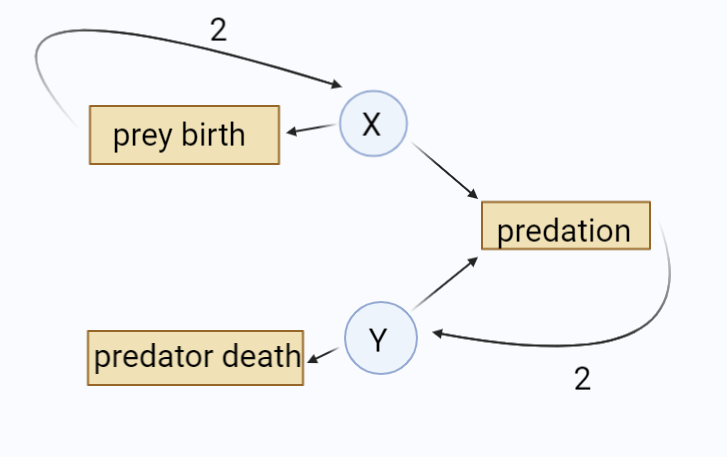
\includegraphics[scale = 0.6]{system_graph.PNG}
  \caption{Graphical representation of the predator-prey model in the hare (X) and lynx (Y) populations as described by the above equations (1-3). Note that the prey birth increases the population of X while predation increases the population of Y }
  \label{fig:systemGraph}
\end{figure}

The vectors of the above Petri net are: 

\begin{equation}
    s = \begin{pmatrix}X\\Y\end{pmatrix},   r = \begin{pmatrix}prey birth\\predation\\ predator death\end{pmatrix}
\end{equation}
 which result in the following input and output matrices: 
 
 \begin{equation}
    W^s^r = \begin{pmatrix}1 & 0\\1 & 1 \\ 0 & 1 \end{pmatrix},   W^r^s = \begin{pmatrix}2 & 0\\0 & 2\\ 0 & 0\end{pmatrix}
\end{equation}

and the resultant stoichiometry matrix of:
\begin{equation}
    S^T = \begin{pmatrix}1 & -1 & 0\\0 & 1 & -1 \end{pmatrix}
\end{equation}
Given the above derived stoichiometry matrix, the construction of the set of ordinary differential equations follows using: 
\begin{equation}
    \frac{d}{dt} \begin{pmatrix}X\\Y \end{pmatrix} = Sh
\end{equation}

where $h$ is the rate vector. Using mass action kinetics the rate vector $h$ can be obtained as follows: 

\begin{equation}
    h = \begin{pmatrix}k_1X\\k_2XY\\k_3Y \end{pmatrix}
\end{equation}

Accordingly the ordinary differential equations is constructed: 
\begin{equation}
    \frac{d}{dt} \begin{pmatrix}X\\Y \end{pmatrix} = \begin{pmatrix}1 & -1 & 0\\0 & 1 & -1 \end{pmatrix} \begin{pmatrix}k_1X\\k_2XY\\k_3Y \end{pmatrix}
\end{equation}

giving rise to the coupled differential equations of the Lotka-Volterra model:

\begin{equation}
    \frac{dX}{dt} = k_1X - k_2XY
\end{equation}
\begin{equation}
    \frac{dY}{dt} = k_2XY - k_3Y
\end{equation}

\subsection{The Lotka-Volterra Model Assumptions}
The Lotka-Volterra model makes several key simplifications in order to grasp the macro-level interactions in the biological system. However, these simplifications rest on several assumptions. 

When looking a the rate of prey population growth this parameter has been simplifies down to equate to prey birth rates. This ignores several important biological limitations on the prey reproduction including rates of sexual maturation, litter mortality rates, and probability of survival to adulthood. In short, it assumes that the growth of the prey population can be succinctly condensed into a single parameter of prey birth rate. 

In a similar manner, the predation interaction term in the model makes a key simplifying assumption. The interaction term here, by virtue of being a two-species population dynamics model, assumes a direct link between the lynx consuming a hare and the growth of the lynx population. That is to say that the reproduction of the lynx population is suggested to be dependent on the number of hares consumed. This is a simplification as the lynx population are known to have a wider and more varied diet, and the hares are known to have a wider array of predators within their ecosystem \parencite{king_geometry_2001, stenseth_population_1997}. Therefore, the interaction term assumes that the only source of energy for lynx reproduction is the predation on hares. The omission of a prey death term also creates an assumption that the only possible cause of death in this system is predation. 

While these simplifications may abstract away from the complexity of the larger ecosystem they allow for the oscillatory dynamics of the two species to be derived in an approachable way. This creates a basis from which nuances and complexities can be built upon. Some of these assumptions, such as the only cause of prey death being predation are also relatively representative heuristics. Indeed, other forms of prey death - such as litter mortality - can be accounted for by adjusting down the prey birth parameter for prey population growth. In this way, these assumptions allow the model to achieve a parsimonious account of the biological system - a powerful tool. 

\section{Code Listings}
The report was conducted using the following MATLAB file: $lynx_hare.mat$ .

This script runs with a local function to encode the model. it runs the ode45 solver and plots the output appropriately. 

These files along with the dataset used can be found stored openly on GITHUB at LINK alongside the LaTeX file used to generate the report itself. 

\section{Extended Discussion}
\subsection{Exploring the Lotka-Volterra Model}
\subsubsection{Cross-checks and model testing}
The Lotka-Volterra model was encoded using MATLAB's ode45 solver. This was coded to simulate the population dynamics and to allow comparison to the historical dataset inferred from the fur pelt records. 

The model was initially established with the following parameter values:
\begin{itemize}
     \item Rate of prey birth: k1 = 1.1
     \item Rate of predation: k2 = 0.001
     \item Rate of predator birth: k3 = 10
     \item Initial populations: 15,000 prey, 1,000 predators
   \end{itemize}

The simulations emerging from these parameter values is depicted in Fig. \ref{fig:intialModel}. Note the correspondence between the growth of predator populations and the decline in prey populations reflecting the interaction between predation and predator population growth over time. This oscillations suggest that the model is behaving as expected in the first instance and accurately reflects the interactions between the prey and predator populations in this system. 

\begin{figure}[H]
  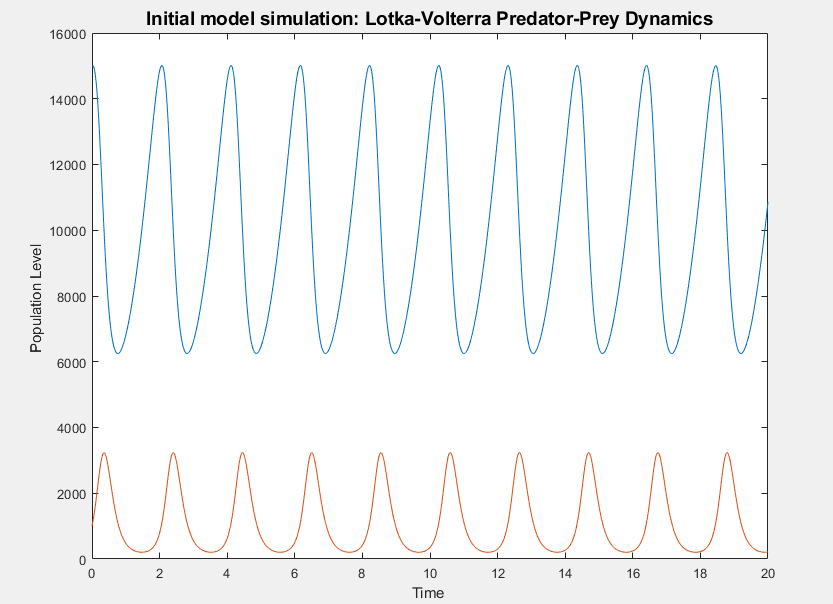
\includegraphics[scale = 0.6]{initial_model.PNG}
  \caption{Graph of the initial parameters values used to simulate the predator-prey dynamic as described by the Lotka-Volterra model. Blue line indicates the prey population oscillations, red line indicates the corresponding predator population oscillations.}
  \label{fig:intialModel}
\end{figure}

To further verify that the system is working as expected the behaviour of the model was examined with different starting points. Of particular interest is the behaviour of the model when either the prey and predator population levels are set to zero. These dynamics are shown in Fig. \ref{fig:testing_start_values}. When there are no predators in the system, as shown in the upper panel of Fig. \ref{fig:testing_start_values}, the prey population grows exponentially. This is expected as the only constraint on the prey population is assumed to be the presence of predation. Conversely, as shown in the lower panel of Fig. \ref{fig:testing_start_values}, the predator population dies off in the absence of any prey. This is expected as without available prey, assumed in this model to be the sole food source for the predators, the predator population cannot survive or reproduce. 

\begin{figure}[H]
    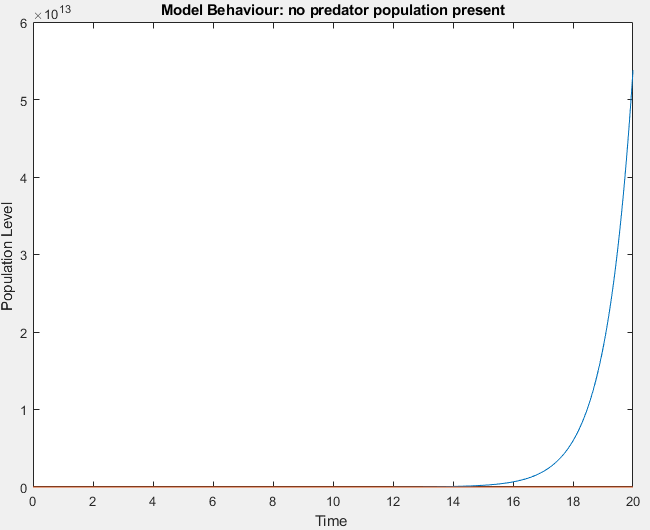
\includegraphics[scale = 0.6]{no_predator.PNG}
    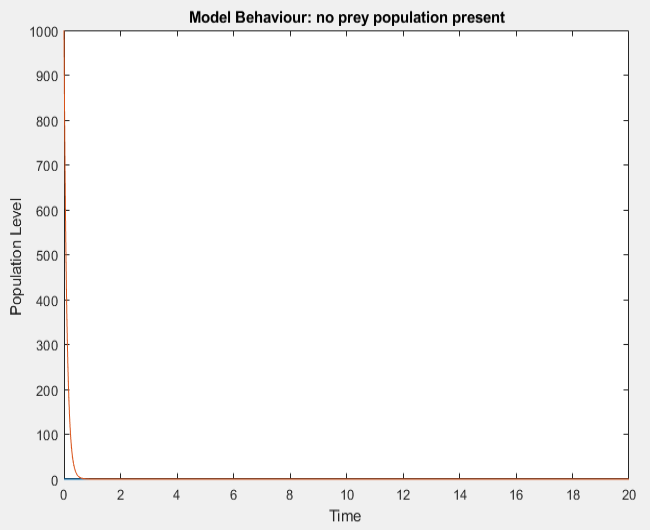
\includegraphics[scale = 0.6]{no_prey.PNG}
    \caption{The upper panel represents the dynamics of the system overtime when the population of predators is set to zero. The prey population grows exponentially over time. In the lower panel the dynamics of the system when the prey population is set to zero are shown. The predator population dies off exponentially over time. In both figures, the blue line indicates the prey population oscillations, red line indicates the corresponding predator population oscillations.}
    \label{fig:testing_start_values}
\end{figure}

\subsubsection{Steady states and Model Exploration}
To identify the model steady states, where the populations are stable, the values at which result in he coupled differential equations of the Lotka-Volterra model equate to zero. 

\begin{eqnarray*}
    \frac{dX}{dt} = k_1X - k_2XY = 0 
\end{eqnarray*}
\begin{eqnarray*}
    X ( k_1 - k_2Y ) = 0  
\end{eqnarray*}
\begin{equation}
    X = 0, Y = k_1 / k_2
\end{equation}

\begin{eqnarray*}
     \frac{dY}{dt} = k_2XY - k_3Y = 0
\end{eqnarray*}
\begin{eqnarray*}
   Y ( k_2X - k_3 ) = 0
\end{eqnarray*}
\begin{equation}
    Y = 0, X = k_3 / k_2
\end{equation}

These values were checked by running the model using these values $X = k_3 / k_2$ and $Y = k_1 / k_2$. The results are shown in Fig. \ref{fig:steady_states}. This demonstrate the system being stable at given values with steady state population of the prey, $X_s_s$, at 10,000, and the steady state population of predators, $Y_s_s$, at 1,100.

\begin{figure}[H]
    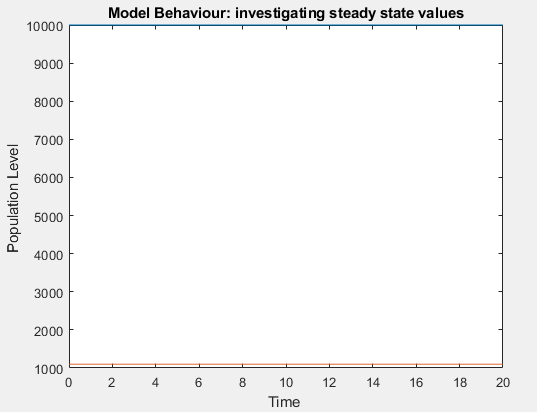
\includegraphics[width=\textwidth]{steady_state.PNG}
    \caption{The steady state populations: $X_s_s$ is 10,000, $Y_s_s$ is 1,100. The blue line indicates the prey population $X_s_s$, red line indicates the corresponding predator population $Y_s_s$.}
    \label{fig:steady_states}
\end{figure}

The effects on the system when the initial conditions are systematically varied, moving them away from the steady state values while leaving the rate constants unchanged, were investigated. The results are shown in Fig. \ref{fig:testing_inital_vals}. With increased perturbation of the start values the amplitude of the population cycles increase. An amplitude of ~300 in observed with a perturbation of 100 on the initial values, rising to a amplitude of ~4300 when the perturbation is set to 1000.
The period of each cycle is also affected, but the effects are less pronounced. The initial perturbation off the steady states of 100 creates a population cycle period of approximately 2 years, when the perturbation is increased to 1000 that period is reduced to 1.9 years. 

\begin{figure}[H]
    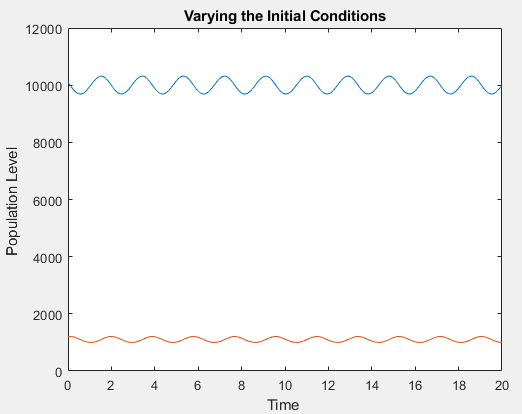
\includegraphics[scale = 0.74]{initial_perb_small.PNG}
    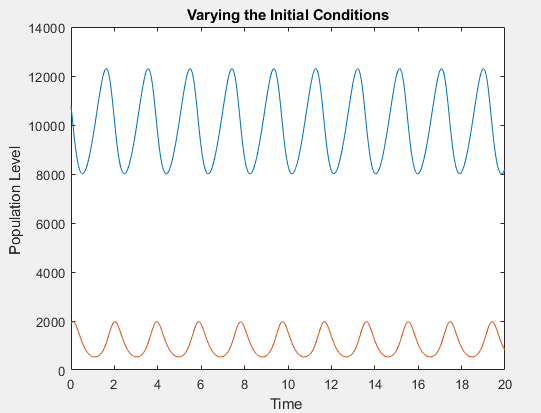
\includegraphics[scale = 0.712]{initial_perb_big.PNG}
    \caption{The upper panel represents the dynamics of the system when the initial values are perturbed by 100. In the lower panel the dynamics of the system when the initial values are perturbed by 1000 are shown. With increased perturbation the amplitude of the population cycles increase and the period of the cycles decrease. In both figures, the blue line indicates the prey population oscillations, red line indicates the corresponding predator population oscillations.}
    \label{fig:testing_inital_vals}
\end{figure}

To explore the effects of changing the rate constants, the model was reset to the steady state population levels.  
The values of the rate constants were systematically varied, beginning with $k_1$ the prey birth rate. 

Results of the variation of $k_1$ are shown in Fig. \ref{fig:k1_vals}. Decreasing the value of $k_1$ results in population cycles of greater amplitude oscillating between 9,000-11,000 (around the $X_s_s$ of 10,000). The predator population is also reduced, oscillating between 550-1,100 (down from the $Y_s_s$ of 1,100). Increasing the value of $k_1$ results in similar fluctuations of the prey species, with amplitudes of 9,200-11,000 (above the $X_s_s$ of 10,000), the predator population also increases, fluctuating between 1000-1,800 (above the $Y_s_s$ of 1,100). These changes are expected, decreasing prey birth pulls down the oscillations for both species, increasing prey birth pushes them upward. 

Looking at $k_2$, predation rate, the results are shown in Fig. \ref{fig:k2_vals}. Lowering $k_2$ results in upward oscillations of prey, 10,000 - 16,000 - and of the predator population 800 - 2,200. Increasing $k_2$ results in downward trending oscillations of the prey population 7,000 - 10,000 and a decreased amplitude of cycle of the predator population. This is also a set of expected effects on the system. Decreasing predation allows the prey population to increase, which in turn allows the predator population to oscillate higher. Similarly, increasing the predation rate puts strain on the prey population and decreases the number of predators the system can support. 

Finally, the effects of varying $k_3$ values, the predator death rate, are shown in Fig. \ref{fig:k3_vals}. Lowering $k_3$ results in an upwards trend in the amplitudes of the predator population 1,000 - 2,000 and a downwards trend in the prey population 6,500 - 10,000. Conversely, increasing predator death sees increases in prey population, 10,000 - 14,000, and a downward trend in predator population amplitudes, 500 - 1,500. Tease are sensible trends to see given that the predator death rate is the only parameter preventing the predator population from growing exponentially and the changing in that parameter will have consequences for the prey population too.   



\begin{figure}[H]
    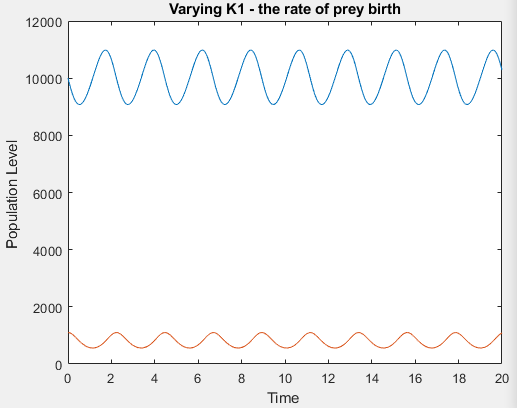
\includegraphics[scale = 0.81]{k1_low.PNG}
    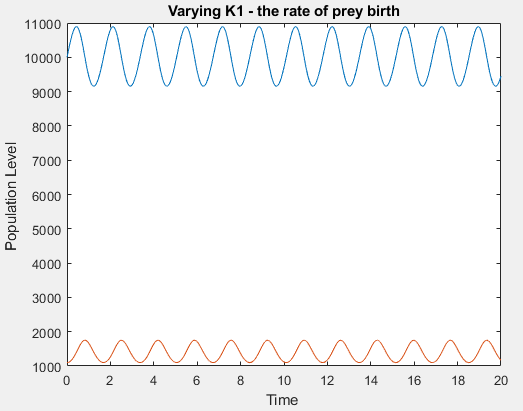
\includegraphics[scale = 0.8]{k1_high.PNG}
    \caption{The upper panel represents the dynamics of the system when the value of $k_1$ is decreased from the initial value of 1.1 to 0.8. The lower panel illustrates the dynamics of the system when the value of $k_1$ is increased from the initial value of 1.1 to 1.4. In both figures, the blue line indicates the prey population oscillations, red line indicates the corresponding predator population oscillations.}
    \label{fig:k1_vals}
\end{figure}

\begin{figure}[H]
    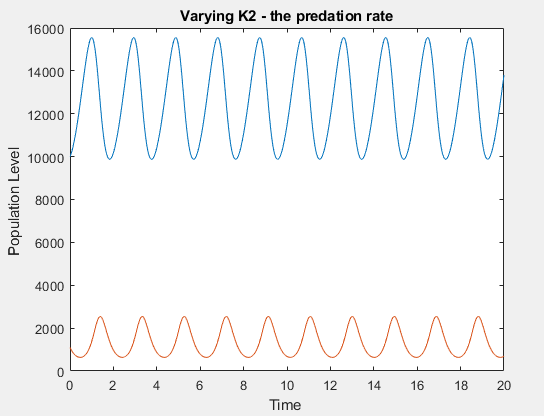
\includegraphics[scale = 0.7]{k2_low.PNG}
    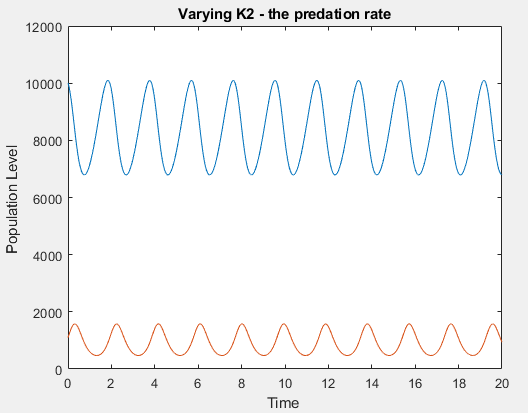
\includegraphics[scale = 0.725]{k2_high.PNG}
    \caption{The upper panel represents the dynamics of the system when the value of $k_2$ is decreased from the initial value of 0.001 to 0.0008. The lower panel illustrates the dynamics of the system when the value of $k_2$ is increased from the initial value of 0.001 to 0.0012. In both figures, the blue line indicates the prey population oscillations, red line indicates the corresponding predator population oscillations.}
    \label{fig:k2_vals}
\end{figure}


\begin{figure}[H]
    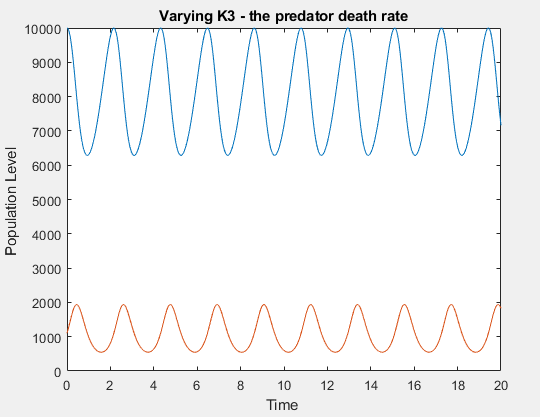
\includegraphics[scale = 0.8]{k3_low.PNG}
    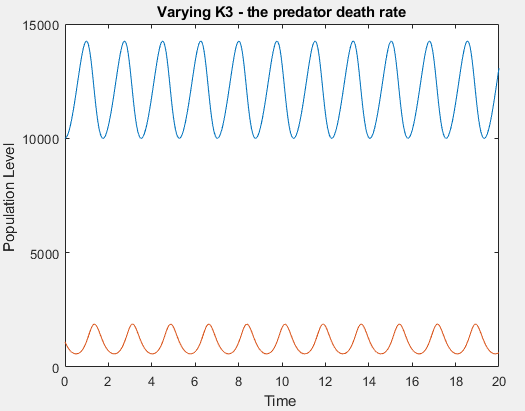
\includegraphics[scale = 0.82]{k3_high.PNG}
    \caption{The upper panel represents the dynamics of the system when the value of $k_3$ is decreased from the initial value of 10 to 8. The lower panel illustrates the dynamics of the system when the value of $k_3$ is increased from the initial value of 10 to 12. In both figures, the blue line indicates the prey population oscillations, red line indicates the corresponding predator population oscillations.}
    \label{fig:k3_vals}
\end{figure}

The exploration of the model, the effects of changing the presence or abscence of each species, the changing of the initial values, the investigation of the rate constants all indicate that the Lotka-Volterra model is a good fit to the population dynamics we wish to describe.

\subsection{Fit the model to the Hare-Lynx Data}
To fit the model to the historical data, biologically plausible estimates of the rate constants need to be derived and input into the model. Consider first the parameter $k_1$, prey birth. In the absence of predation the prey population should grow exponentially according to the following equation: 

\begin{equation}
    X(t) = X_0e^{k_1t}
\end{equation}

This allows an ecologically valid estimate of the $k_1$ point range to be derived. Consider that $N_0$ is the number of hares at the start of a year, for breeding to occur $N_0$ must be 2. The average litter size $L_s$ is 3, and the average number of litters per year $L_n$ is 2.6.The number of new offspring, $N_n_e_w$, assuming all survive is therefore $L_s$*$L_n$.

After one year, the number of hares can be described as follows:
\begin{equation*}
    N_1 = N_0 + N_n_e_w
\end{equation*}
However, consider from the previous equation that $N_1$ is equivalent to $X(t)$, therefore:
\begin{equation*}
    N1 = N0 * e^{k_1t}
\end{equation*}
Resulting in the following:
\begin{equation*}
    N_0 + N_n_e_w = N0e^{k_1t}
\end{equation*}
Here t=1, as 1 year has passed, so the equation can be evaluated as follows: 
\begin{equation*}
    log_N_0(N_0 + N_n_e_w) = k_1
\end{equation*}

For maximum population growth (assuming no offspring mortality, maximum litters and maximum offspring per litter) $k_1$ is found to be $log_N_0(N_0 + N_n_e_w)$ where $N_0$ is the value of the population at the beginning of the year $t$.Taking again the biologically plausible values for the reproduction rates of the hares we find that $t = 1$, a breeding pair would have had a maximum of $7.8$ offspring. This means that at the biologically plausible maximum the value for $k_1$ is at:
\begin{equation}
    k_1 = log_2(9.8) = 3.26
\end{equation}

Evaluating on whole numbers from $0-7$, we find the an ecologically plausible point range for $k_1$ is $[1.0, 1.5855, 2, 2.32, 2.585, 2.807, 3.0, 3.169]$. 

Assuming that the fur pelt record is an accurate measure of species populations, an ecologically valid estimate of the steady state of the populations can be inferred from graphing the pelt oscillations, as populations oscillate around their steady state values. Visual evaluation of Fig. \ref{fig:pelt_record} indicates that the hare population steady state sits around $50,000$, however the mean of the data is $X_s_s = 34081$ and that lynx population sits near $30,000$, however, the mean of the data is $Y_s_s = 20167$. 

\begin{figure}[H]
    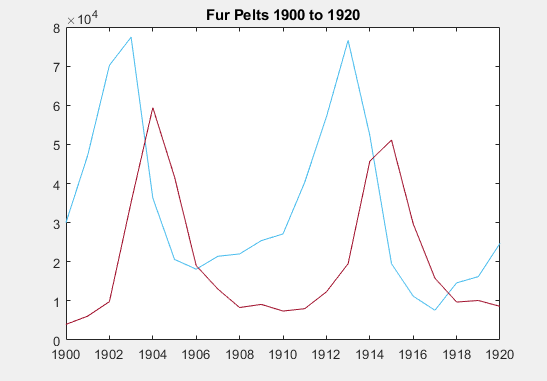
\includegraphics[width = \textwidth]{fur_pelts.PNG}
    \caption{The data from the pelt trapping records from 1900-1920 of the snow hare and canada lynx pelts. The blue line indicates the prey (hare) pelt oscillations, red line indicates the corresponding predator (lynx) pelt oscillations.}
    \label{fig:pelt_record}
\end{figure}

Given that we have a point range of ecological estimates for $k_1$, of which we can take the median value, these steady states allow an inference on the values of $k_2$ and $k_3$ respectively. 

\begin{equation}
    k_1 = median[1.0, 1.5855, 2, 2.32, 2.585, 2.807, 3.0, 3.169] = 2.585
\end{equation}
\begin{equation}
    k_2 = \frac{k_1}{Y_s_s} = \frac{2.4525}{30000} = 0.00008175
\end{equation}
\begin{equation}
    k_3 = k_1\frac{X_s_s}{Y_s_s} = 2.4525*\frac{50000}{30000} = 4.0875
\end{equation}

Taking these values for the rate parameters, and the start values from the pelt data at 1900 we can simulate the model for the same time period and see how it compares to Fig. \ref{fig:pelt_record}.

\subsubsection{Model Behaviour and Preliminary Results}
The initial model simulation does not approximate the historical data well using these constants, Fig. \ref{fig:results_1}. The amplitude of the cycles of both populations are reasonable approximations of the historical data but the period of the population cycles is too short, lasting only a few years, not a decade or more.  
\begin{figure}[H]
    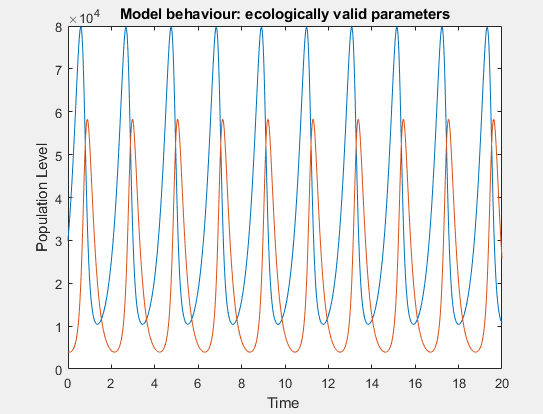
\includegraphics[width = \textwidth]{results_1.PNG}
    \caption{Initial model simulation using historical start values, $k_1 = 2.585$, $k_2 = 0.00008$, $k_3 = 4.0874$. The blue line indicates the prey (hare) pelt oscillations, red line indicates the corresponding predator (lynx) pelt oscillations. Note that the amplitude of the cycles maps well to the historical data but the period is much too short.}
    \label{fig:results_1}
\end{figure}

Considering again the meaning of the rate parameters - $k_1$ could be considered more holistically as the population growth parameter of the prey. At present and in Fig. \ref{fig:results_1} $k_1$ and the resultant values for $k_2$ and $k_3$ are based on the population birth rate. However, the population growth should include mortality and survival outside of predation too. Therefore, lowering $k_1$ and in turn changing the values of $k_2$ and $k_3$ may help the model fit more accurately to the historical pelt record. 
Both male and female snowshoe hares are known to reach sexual maturity only at about 1 year of age, they also only have a longevity of approximately 3 years in total - both of these factors will slow the population growth rate of the species. Consider further the fact that while the lynx preys almost exclusively on the hare population, the snowshoe hares have many predators. Accordingly the value of $k_1$ was reduced significantly in a refit as shown in Fig. \ref{fig:results_2}. Mapping the simulated model to the historical data indicates just how strong a fit the model has created to the historical pelt data, see Fig. \ref{fig:results_3}.

\begin{figure}[H]
    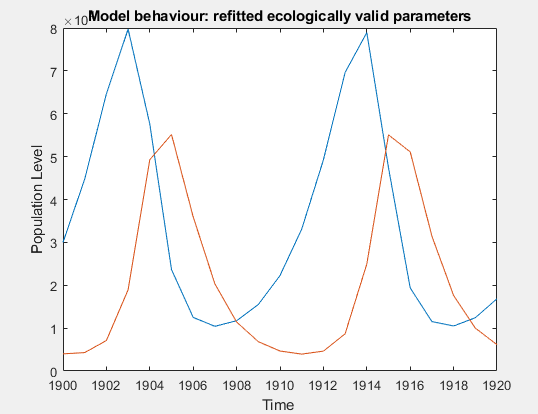
\includegraphics[width = \textwidth]{results_2.PNG}
    \caption{Refit of model simulation using historical start values, $k_1 = 0.5$, $k_2 = 2.5e^-5$, $k_3 = 0.845$. The blue line indicates the prey (hare) pelt oscillations, red line indicates the corresponding predator (lynx) pelt oscillations. Note that amplitude and period of the model simulation now seem to approximate the historical data well.}
    \label{fig:results_2}
\end{figure}

\begin{figure}[H]
    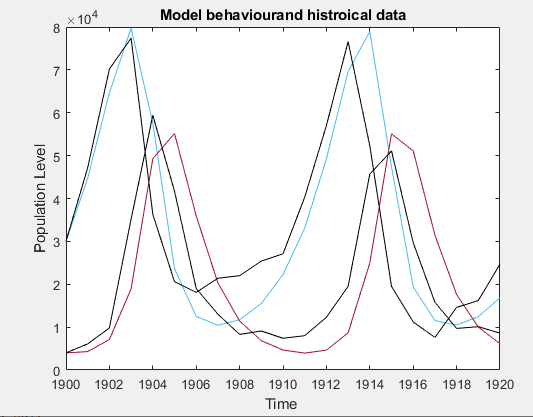
\includegraphics[width = \textwidth]{results_3.PNG}
    \caption{Overlay of model simulations and historical data. The historical data is presented in black. The model simulations are plotted in blue and red for the prey and predator populations, respectively. Note the close fit of the simulations to the historical pelt data.}
    \label{fig:results_3}
\end{figure}

\subsubsection{Model Extensions}

 
\subsection{Relating findings to the biological system}

Looking at the cycles in the system it is clear that the snow hare population appears to reach a peak before falling in numbers. Research suggest this is due to food limitation, and that similarly the subsequent decline is due to predation \parencite{king_geometry_2001}. These factors are supported by field experiment results where hare populations were given extra food and refuge from predation which 


\subsection{Critical discussion: Limitations, assumptions and future steps}

The model is also limited by its inclusion of just two species - the food web of even the more sparse ecosystem of the boreal forest is still more complex than this model projects \parencite{stenseth_population_1997} - see Fig. \ref{fig:food_web} for details.

\begin{figure}[H]
    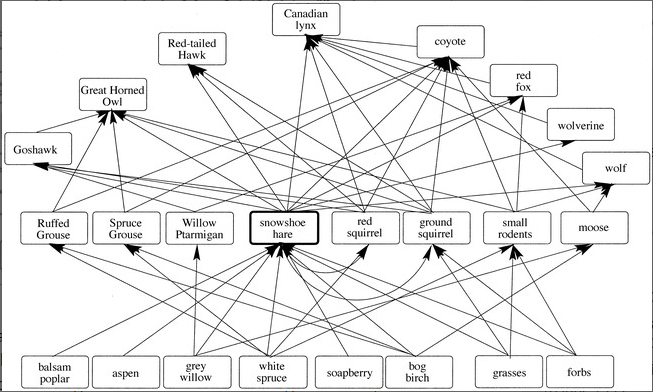
\includegraphics[width = \textwidth]{food_web.PNG}
    \caption{Food web of the Candian boreal forest - taken from \parencite{king_geometry_2001}}
    \label{fig:food_web}
\end{figure}

\section{Outlook}

\clearpage
\section{References}
\printbibliography
\end{document}
